\documentclass{beamer}
\special{landscape}

\usetheme{Warsaw}

%\usecolortheme{seahorse}
%\usefonttheme[onlysmall]{structurebold}

\setbeamertemplate{headline}[split]
\setbeamertemplate{footline}[default]
\setbeamertemplate{footline}[miniframes theme]
%\logo{\includegraphics[scale=0.25]{lifia_logo.png}}

\mode<presentation>
\usepackage[spanish]{babel}
\usepackage{beamerthemesplit}
\usepackage{color}      % use if color is used in text

\usepackage[utf8]{inputenc}

% Comandos en modo Verbatim
%\usepackage{fancyvrb}

\usepackage{listings}


\lstdefinelanguage[mips]{Assembler}{%
  sensitive=false,%
  morecomment=[l]{;},%
  % so listings can detect directives and register names
  alsoletter={.\$},
  % strings, characters, and comments
  morestring=[b]",
  morestring=[b]',
  morecomment=[l]\#,
  numberstyle=\color{green},
  % instructions
  morekeywords={[1]cvt.l.d,cvt.d.l,mfc1,mtc1,DADD,DADDI,ANDI,XORI,HALT,BEQ,BNEQ,LD,NOP,DMUL,DSUB,AND,DDIV,%
	JAL,J,DSLL,BNEZ,SD, JR, BEQZ, cvt.d.l, cvt.l.d, lwu},
  % assembler directives
  morekeywords={[2].word,.code,.data, .asciiz, .ascii, .word32},
  % register names
  morekeywords={[3]F0,F1,F2,F3,F4,F5,F6,F7,F8,F9,F10,F11,F12,F13,F14,F15,F16,F17,F18,F19,%
    F20,F21,F22,F23,F24,F25,F26,F27,F28,F29,F30,F31,%
    f0,f1,f2,f3,f4,f5,f6,f7,f8,f9,f10,f11,f12,f13,f14,f15,f16,f17,f18,f19,%
    f20,f21,f22,f23,f24,f25,f26,f27,f28,f29,f30,f31,%
    R0,R1,R2,R3,R4,R5,R6,R7,R8,R9,R10,R11,R12,R13,R14,R15,R16,R17,R18,R19,%
    R20,R21,R22,R23,R24,R25,R26,R27,R28,R29,R30,R31,%
    r0,r1,r2,r3,r4,r5,r6,r7,r8,r9,r10,r11,r12,r13,r14,r15,r16,r17,r18,r19,%
    r20,r21,r22,r23,r24,r25,r26,r27,r28,r29,r30,r31,%
	\$0,\$zero,\$s0,$s1,$s2,$s3,$s4,$s5,$s6,$s7,$sp,$ra,$t0,$t1,$t2,$t3,$t4,$t5,$t6,$t7,$t8,$t9,%
	$sp,$a0,$a1,$a2,$a3,$v0,$v1%
    },
  keywordstyle=\color{green},
  keywordstyle=[2]\color{blue},% for example
  keywordstyle=[2]\color{blue},% for example
  keywordstyle=[3]\color{red},% for example
 }[strings,comments,keywords]


\definecolor{CommentGreen}{rgb}{0,.6,0}
\lstset{
   language=[mips]Assembler,
   escapechar=@, % include LaTeX code between `@' characters
   keepspaces,   % needed to preserve spacing with lstinline
   basicstyle=\footnotesize\ttfamily\bfseries,
   commentstyle=\color{CommentGreen},
   stringstyle=\color{cyan},
   showstringspaces=false,
   keywordstyle=[1]\color{blue},    % instructions
   keywordstyle=[2]\color{magenta}, % directives
   keywordstyle=[3]\color{red},     % registers
%  numbers=left,
%  numbersep=15pt,
%  numberstyle=\tiny\color{green},
 }

%%
%% WinMIPS64 definition (c) 2020
%\lstdefinelanguage{WinMIPS64_old}
% {keywords={%
%cvt.l.d,cvt.d.l,mfc1,mtc1,DADD,DADDI,ANDI,XORI,HALT,BEQ,BNEQ,LD,NOP,DMUL,DSUB,AND,DDIV,%
%	JAL,J,DSLL,BNEZ,SD, JR, BEQZ, cvt.d.l, cvt.l.d, lwu},%
% otherkeywords={.word,.code,.data,.code, .asciiz, .ascii, .word32 },%
%   sensitive=false,%
%   morecomment=[l]{;},%
%   morestring=[b]",%
%   keywordstyle=\color{green},
%  keywordstyle=[2]\color{brown},% for example
% }

%\lstset{emph={%
%    F0,F1,F2,F3,F4,F5,F6,F7,F8,F9,F10,F11,F12,F13,F14,F15,F16,F17,F18,F19,%
%    F20,F21,F22,F23,F24,F25,F26,F27,F28,F29,F30,F31,%
%    f0,f1,f2,f3,f4,f5,f6,f7,f8,f9,f10,f11,f12,f13,f14,f15,f16,f17,f18,f19,%
%    f20,f21,f22,f23,f24,f25,f26,f27,f28,f29,f30,f31,%
%    R0,R1,R2,R3,R4,R5,R6,R7,R8,R9,R10,R11,R12,R13,R14,R15,R16,R17,R18,R19,%
%    R20,R21,R22,R23,R24,R25,R26,R27,R28,R29,R30,R31,%
%    r0,r1,r2,r3,r4,r5,r6,r7,r8,r9,r10,r11,r12,r13,r14,r15,r16,r17,r18,r19,%
%    r20,r21,r22,r23,r24,r25,r26,r27,r28,r29,r30,r31,%
%	\$0,\$zero,\$s0,$s1,$s2,$s3,$s4,$s5,$s6,$s7,$sp,$ra,$t0,$t1,$t2,$t3,$t4,$t5,$t6,$t7,$t8,$t9,%
%	$sp,$a0,$a1,$a2,$a3,$v0,$v1%
%    },emphstyle={\color{red}\bfseries}%
%}%

%\lstset{emph={%
%    .code,.data,.word
%    },emphstyle={\color{green}\bfseries}%
%}%

\title{Practica 6 - WinMIPS64}
%\author{Juan Antonio Zubimendi\\azubimendi@lifia.info.unlp.edu.ar}

\AtBeginSection[]

\begin{document}

\section{Atascos}


\begin{frame}
\frametitle{Atascos}
Llamamos \emph{atasco} a la situación que impide a una o mas instrucciones seguir su camino en el cauce.

\begin{itemize}
\item Estructural
\begin{itemize}
\item Provocados por conflictos con los recursos.
\end{itemize}


\item Dependencia de Datos
\begin{itemize}
\item Dos instrucciones se comunican por medio de un dato
\end{itemize}

\item Dependencia de Control
\begin{itemize}
\item La ejecución de una instrucción depende de cómo se ejecute otra
\end{itemize}

\end{itemize}
Si resolvemos con paradas del cauce, disminuye el rendimiento teórico
\end{frame}

\section{Atascos por dependencia de Datos}
\subsection{General}

\begin{frame}
\frametitle{Atasco por Dependencia de Datos}

Condición en la que los operandos fuente o destino de una instrucción no están disponibles en el momento en que se necesitan en una etapa determinada del cauce.
\begin{itemize}

\item Lectura después de Escritura (RAW, dependencia verdadera)
\begin{itemize}
\item  una instrucción genera un dato que lee otra posterior
\end{itemize}

\item Escritura después de Escritura (WAW, dependencia en salida)
\begin{itemize}
\item una instrucción escribe un dato después que otra posterior
\item sólo se da si se deja que las instrucciones se adelanten unas a otras
\end{itemize}

\item Escritura después de Lectura (WAR, antidependencia)
\begin{itemize}
\item una instrucción modifica un valor antes de que otra anterior que lo tiene que leer lo lea
\item Es el que menos suele darse
\end{itemize}
\end{itemize}
\end{frame}


\subsection{WAW - Escritura luego de una Escritura}
\begin{frame}[fragile]
\frametitle{WAW}
Una instrucción escribe un dato después que otra posterior
\begin{block}{}
\begin{lstlisting}[basicstyle=\ttfamily,keywordstyle=\color{blue}]
.code

dmul r1,r2,r3
dadd r1,r6,r3
halt
\end{lstlisting}
\end{block}

\end{frame}


\begin{frame}[fragile]
\frametitle{WAW}
Una instrucción escribe un dato después que otra posterior
\begin{block}{}
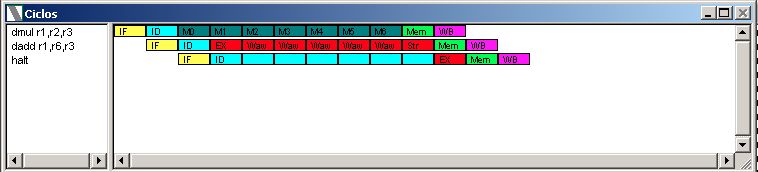
\includegraphics[scale=0.45]{waw.png}
\end{block}
\end{frame}

\subsection{WAR - Escritura luego de una Lectura}
\begin{frame}[fragile]
\frametitle{WAR}
Una instrucción escribe el valor de un registro antes que otra anterior que lo tiene que leer lo lea
\begin{block}{}
\begin{lstlisting}[basicstyle=\ttfamily,keywordstyle=\color{blue}]
.code ; Activar Forwarding

dmul r7,r1,r3
dmul r10,r7,r4
dadd r4,r5,r6
halt
\end{lstlisting}
\end{block}

\end{frame}


\begin{frame}[fragile]
\frametitle{WAR}
Una instrucción escribe el valor de un registro antes que otra anterior que lo tiene que leer lo lea
\begin{block}{}
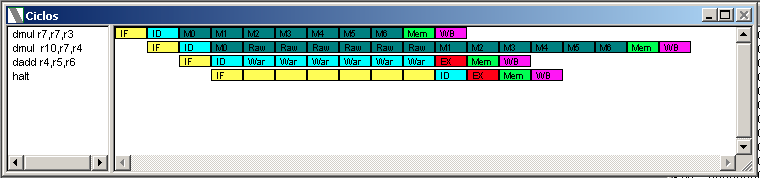
\includegraphics[scale=0.45]{war.png}
\end{block}
\end{frame}



\section{Atascos Estructurales}

\begin{frame}[fragile]
\frametitle{Atascos Estructurales}
Dos o mas instrucciones necesitan utilizar el mismo recurso hardware en el mismo ciclo.

\begin{block}{}
\begin{lstlisting}[basicstyle=\ttfamily,keywordstyle=\color{blue}]
.code
dmul r7,r7,r3
nop
nop
nop
nop
nop
halt
\end{lstlisting}
\end{block}
\end{frame}

\begin{frame}[fragile]
\frametitle{Atasco Estructural}
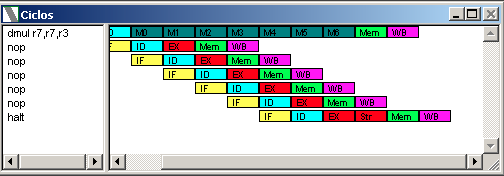
\includegraphics[scale=0.45]{atasco-estructural.png}
\end{frame}


\section{Posibles soluciones a riesgos estructurales}
\begin{frame}
\frametitle{Soluciones a riesgos estructurales}
Replicar, segmentar ó realizar turnos para el acceso a las unidades funcionales en conflicto.
\begin{itemize}
\item Duplicación de recursos hardware
\begin{itemize}
\item Unidades separadas para multiplicar, dividir además de la ALU
\end{itemize}
\item Separación en memorias de instrucciones y datos
\item Turnar el acceso al banco de registros
\begin{itemize}
\item Escrituras en la primera mitad de los ciclos de reloj
\item Lecturas en la segunda mitad de los ciclos de reloj
\end{itemize}
\end{itemize}
\end{frame}



\end{document}

